%***********************************************************************
% PREÁMBULO:
%***********************************************************************
%
% Contiene:
%   - La clase de documento que se va a generar (\documentclass).
%   - Las declaraciones de los paquetes que se van a usar (\usepackage).
%   - Las definiciones de nuevos comandos y entornos (\newcommand y \newenvironment).
%   - Referencia a órdenes (uso de comandos) que van a afectar a todo el documento.
% 
%_______________________________________________________________________

    
    % IMPORTANTE: De aquí en adelante, las siglas «SCS» se refieren al «Sistema de Computación Set».


    % NOTA: Muchos de los comentarios explicativos que aparecen a continuación, sobre los paquetes usados y comandos definidos para la generación de la documentación del SCS, han sido extraídos de fragmentos del libro siguiente: «El libro de LaTeX, de Bernardo Cascales, Pascual Lucas, José Manuel Mira, Antonio Pallarés y Salvador Sánchez-Pedreño. Prentice Hall, 2003».


    % Para la la generación de la documentación del SCS se utiliza la clase de documento book porque proveé los siguientes tres grandes bloques: la unidad «frontal», la «principal» y la «posterior» que se especifican con los comandos \frontmatter, \mainmatter y \backmatter respectivamente. La primera de ellas contendrá todas las posibles «páginas de título» (portadilla, portada, página de derechos, dedicatoria, lema, etc.), los prólogos, el índice general, los índices de cuadros y figuras... La parte principal contendrá el contenido del libro propiamente dicho y los apéndices. Finalmente la unidad posterior estaría ocupada por los anexos, bibliografía e índices alfabéticos.
    \documentclass[10pt,a4paper,final,twoside,openright,onecolumn,titlepage]{book}
    % Las opciones utilizadas para la clase book tienen el siguiente significado:

        % - 10pt, establece el tamaño del texto normal (el determinado con el comando \normalsize) en 10 puntos de impresión.

        % - a4paper, establece el tamaño del papel (de las páginas del pdf) a 210mm x 297mm.
        
        % - final, prohíbe que se marcan en el pdf las líneas en las existe un Overfull; por ejemplo, líneas en las que LateX no sabe como hacer la división silábica  (división de una palabra en dos partes, entre dos de sus sílabas, que a veces se realiza con la última palabra de cada línea). La opción opuesta es draft (borrador).
        
        % - twoside, el documento se prepara para ser impreso a dos caras.
        
        % - openright, especifica que todos los capítulos comenzarán en una nueva página «a derecha». Es decir si LaTeX, al generar un título con el comando chapter, detecta que la nueva página (la siguiente al párrafo anterior a usar \chapter) es una página «a izquierda», entonces introducirá otro salto de página más para que el título del capítulo comience en una nueva página «a derecha».
        
        % onecolumn, indica que el texto será compuesto en una sola columna por página.
        
        % titlepage, con esta opción el comando \maketitle ubicará «la página de título» en una sola página real e independiente y el entorno abstract se comportará del mismo modo respecto a su contenido.


    \usepackage[utf8]{inputenc}% Con este paquete y esta opción le decimos a LaTeX que estamos usando la codificación utf8 del teclado de nuestro computador, válida, por ejemplo, con los sistemas operativos MS-Windows o Linux. Ahora LaTeX reconoce las vocales acentuadas y los demás símbolos del teclado, con lo que evitamos su desaparición del texto.

    \usepackage[T1]{fontenc}% Su uso no es imprescindible y, a diferencia del paquete anterior, no está relacionado con la introducción de caracteres con tildes desde el teclado en un documento, sino con la gestión interna que TeX realiza con las fuentes o «tipos» para producir la salida de tales caracteres acentuados en el documento compilado. Para explicar esto hemos de referirnos a que Donald E. Knuth, además de TeX, creó otro compilador, llamado Metafont. capaz de generar los tipos que TeX utilizaba. En lugar de crear un tipo para, por ejemplo, el carácter 'a', otro para 'á', 'à', etc., optó por crear un tipo para el carácter 'a' y otro para la tilde aguda '´', que puede ser utilizado en diferentes letras. Durante el proceso de compilación TeX produce un tipo como el 'á' que no está disponible, superponiendo al tipo 'a' la tilde aguda. En el caso de disponer de una fuente de tipos en la que los caracteres acentuados existen como tales, no es necesario realizar el proceso de superposición anterior, lo que evita algunos errores de división silábica automática en palabras acentuadas. El paquete fontenc con la opción T1 sirve para indicar a TeX que disponemos de fuentes de tipos con caracteres acentuados (entre otras cosas) y que utilice estos en lugar de construirlos.

    \usepackage[spanish]{babel}% Con este paquete y esta opción le indicamos a LaTeX que vamos a escribir en español. Así, LaTeX se guiará por las reglas del español para la división silábica, e interpretará en nuestro idioma algunos comandos como el utilizado para poner la fechar del día, \today.

    \renewcommand{\shorthandsspanish}{}% Desactivamos todos los métodos tipográficos incluidos con la opción spanish de babel.

    \usepackage[sc,osf]{mathpazo}% Palatino es la fuente principal.
    \linespread{1.05}\selectfont% Palatino necesita un poco de espacio extra, con 1.05 se establece un 5% de espacio extra.
    \usepackage[scaled=.88]{beramono}% Bera para las fuentes monoespaciadas.
    \usepackage[scaled=.86]{berasans}% Bera para las fuentes Sans-Serif.

    \usepackage{marvosym}% Para usar los símbolos: Letter

    \newcommand\abstractname{Abstract}
    \makeatletter% El entorno abstract no existe en la clase book, así que lo definimos de manera similar a como se hace en clase report.cls.
        \if@titlepage
            \newenvironment{abstract}%
            {%
                \titlepage
                \null\vfil
                \@beginparpenalty\@lowpenalty
                \thispagestyle{plain}% Numera la página del abstract .
                \begin{center}%
                \bfseries \abstractname
                \@endparpenalty\@M
                \end{center}%
            }{%
                \par\vfil\null\endtitlepage%
            }%
        \else
            \newenvironment{abstract}%
            {%
                \if@twocolumn
                    \section*{\abstractname}%
                \else
                    \small
                    \begin{center}%
                        {\bfseries \abstractname\vspace{-.5em}\vspace{\z@}}%
                    \end{center}%
                    \quotation
                \fi%
            }{%
                \if@twocolumn\else\endquotation\fi%
            }
        \fi
    \makeatother

    \newcommand{\cod}[1]{{\normalfont\ttfamily\ifFootNote#1\else\small #1\fi}}
    \newcommand{\pat}[1]{{\normalfont\sffamily #1}}
    \newcommand{\sbr}[1]{{\fboxsep0.5pt\colorbox{gray!20}{{\footnotesize\strut}#1}}}

    % Ver sección 7.10.7 del libro «The LaTeX Companion. Tools and Techniques for Computer Typesetting (2nd Edition), by Frank Mittelbach and Michel Goossens (with Johannes Braams, David Carlisle, and Chris Rowley). Addison-Wesley, 2004». Ver la tabla 7.29 «Glyph chart for msbm10 produced by the nfssfont.tex program».
    \DeclareSymbolFont{AMSb}{U}{msb}{m}{n}
        \DeclareMathSymbol{\Natural}{\mathalpha}{AMSb}{'116}
        \DeclareMathSymbol{\Integer}{\mathalpha}{AMSb}{'132}
        \DeclareMathSymbol{\Rational}{\mathalpha}{AMSb}{'121}
        \DeclareMathSymbol{\Real}{\mathalpha}{AMSb}{'122}
        \DeclareMathSymbol{\Complex}{\mathalpha}{AMSb}{'103}
        \DeclareMathSymbol{\String}{\mathalpha}{AMSb}{'123}

    \usepackage{newunicodechar}% Para usar los comandos: \newunicodechar 

    \newcommand{\UnicodeFormat}[1]{\ensuremath{#1}}
        \newunicodechar{ℕ}{\UnicodeFormat{\Natural}}
        \newunicodechar{ℤ}{\UnicodeFormat{\Integer}}
        \newunicodechar{ℚ}{\UnicodeFormat{\Rational}}
        \newunicodechar{ℝ}{\UnicodeFormat{\Real}}
        \newunicodechar{ℂ}{\UnicodeFormat{\Complex}}
        \newunicodechar{𝕊}{\UnicodeFormat{\String}}
        \newunicodechar{←}{\UnicodeFormat{\leftarrow}}
        \newunicodechar{→}{\UnicodeFormat{\rightarrow}}
        \newunicodechar{×}{\UnicodeFormat{\times}}
        \newunicodechar{⋀}{\UnicodeFormat{\land}}
        \newunicodechar{⋁}{\UnicodeFormat{\lor}}
        \newunicodechar{⊻}{\UnicodeFormat{\veebar}}
        \newunicodechar{≠}{\UnicodeFormat{\neq}}
        \newunicodechar{∈}{\UnicodeFormat{\in}}

    \usepackage[usenames,dvipsnames,svgnames,table]{xcolor}% Para usar colores.

    \usepackage{listings}% Para incluir códigos en la documentación. Comandos: \lstdefinestyle, \lstdefinelanguage, \lstlistingname, \lstinputlisting, \lstlistlistingname, \lstlistoflistings

    \renewcommand\lstlistingname{Código}

    \lstdefinestyle{lstGeneralStyle}
    {
        mathescape      = true,
        breaklines      = true,
        breakatwhitespace = true,
        basicstyle      = \small\ttfamily,
        keywordstyle    = \small\bfseries\ttfamily,
        commentstyle    = \color{darkgray}\small\itshape\ttfamily,
        tabsize         = 3,% tres espacios
        columns         = fixed,
        frame           = t,
        rulecolor       = \color{darkgray},
        numbers         = left,
        numbersep       = 7pt,
        numberstyle     = \color{darkgray}\fontfamily{fxl}\selectfont\scriptsize\sffamily,
        %belowskip       = \bigskipamount
    }
    
    \lstdefinelanguage{set}
    {
        style       =lstGeneralStyle,
        keywords    ={end, if, while},
        morecomment =[l]{;},
        morecomment =[s]{;-}{-;},
        literate=%
            {á}{{\'a}}1 {Á}{{\'A}}1%
            {é}{{\'e}}1 {É}{{\'E}}1%
            {í}{{\'i}}1 {Í}{{\'I}}1%
            {ó}{{\'o}}1 {Ó}{{\'O}}1%
            {ú}{{\'u}}1 {Ú}{{\'U}}1%
            {ñ}{{\~n}}1 {Ñ}{{\~N}}1%
            {¡}{{!`}}1 {¿}{{?`}}1%
            {ℕ}{{\ensuremath{\naturales}}}1%
            {ℚ}{{\ensuremath{\racionales}}}1%
            {ℝ}{{\ensuremath{\reales}}}1%
            {𝕊}{{\ensuremath{\cadena}}}1%
            {∈}{{\ensuremath{\in}}}1%
            {→}{{\ensuremath{\rightarrow}}}1%
            {←}{{\ensuremath{\leftarrow}}}1%
            {·}{{\ensuremath{\cdot}}}1%
    }

    \makeatletter
        \newcommand{\getlstname}%
        {%
            \protect\filename@parse{\lstname}%
            \cod{(%\protect\filename@base% Devuelve el nombre del fichero de código incluido con \lstinputlisting.
            .\protect\filename@ext)}% Devuelve la extensión del fichero de código incluido con \lstinputlisting.
        }
    \makeatother

    \usepackage{ragged2e}% Comandos: \RaggedRight

    \makeatletter
        \renewcommand{\@makefnmark}{\hbox{\normalfont\textsuperscript{\fontfamily{fxl}\selectfont\sffamily\@thefnmark}}}% Modifica el aspecto de los superíndices de referencia a las notas al pie de página y en las notas al pie de página
    \makeatother

    \usepackage{dblfnote}% Establece a doble columna las notas al pie de página.
    \DFNcolumnsep=15pt% Separación entre las columnas de las notas al pie de página.
    \skip\footins=12pt plus 4.0pt minus 2.0pt% Espacio que separada el contenido principal de las notas al pie de página.

    \makeatletter
        %\renewcommand\@makefntext[1]{\noindent\@makefnmark#1}% Elimina la indentación de las notas al pie de página.
    \makeatother

    \newif\ifFootNote
    \let\oldfootnote\footnote
    \renewcommand{\footnote}[1]{\FootNotetrue\oldfootnote{\RaggedRight#1}\FootNotefalse}

    \usepackage%
    [%
        linktocpage = false,% El 'hyperlink' se establece sobre el título de la entrada de la tabla de contenido y no sobre el número de página.
        hidelinks,% Elimina el borde color de los links.
    ]{hyperref}% Permite los hyperlinks en el documento pdf y marcadores automáticos. Por ejemplo, permite hacer clic en el superíndice que hace referencia a una nota al pie de página para desplazarnos hacia ella. Comandos: \pdfbookmark

    \usepackage[numbered]{bookmark}% Para numerar los marcadores. Comandos: \bookmark


    % Redefinimos el aspecto de los labels del entorno 'itemize'.
    \renewcommand{\labelitemi}{\textbullet}
    \renewcommand{\labelitemii}{\normalfont\bfseries\textendash}
    \renewcommand{\labelitemiii}{\textperiodcentered}

    \usepackage{microtype}% Para modificar el espacio que hay entre las letras. Las opciones especificadas evitan un error tipográfico que hace los títulos de las secciones queden un poco indentados. Comandos: \textls.

    \DeclareRobustCommand{\mysmallcap}[1]{\scshape\MakeLowercase{#1}}
    \DeclareRobustCommand{\mysmallcapsep}[1]{\textls*[80]{\scshape\MakeLowercase{#1}}}
    \DeclareRobustCommand{\mybigcap}[1]{\MakeUppercase{#1}}
    \DeclareRobustCommand{\mybigcapsep}[1]{\textls*[160]{\MakeUppercase{#1}}}


   % Cuando se usa la opción 'openright' de la clase 'book', que hace que todos los capítulos se inicien en página a derecha, en ocasiones provoca que la página izquierda inmediatamente anterior al inicio del capítulo no contenga nada salvo la cabecera. Para eliminar también la cabecera, redefinimos el comando \cleardoublepage.
    \makeatletter 
        \renewcommand*{\cleardoublepage}%
        {%
            \clearpage%
            \if@twoside%
                \ifodd%
                    \c@page%
                \else%
                    \hbox{}%
                    \thispagestyle{empty}\newpage%
                    \if@twocolumn%
                        \hbox{}\newpage%
                    \fi%
                \fi%
            \fi%
        }%
    \makeatother

    \usepackage{xspace}% Para usar el comando: \xspace
    % Ver: http://tex.stackexchange.com/questions/31091/space-after-latex-commands
    \def\Set{{\normalfont\sffamily Set}\xspace}
    \def\SCS{{\sffamily  Sc\kern-1pt\lower-2.5pt\hbox{s}}\xspace}


    \usepackage{microtype}% Para aumentar la separación entre las letras: Comandos: \lsstyle, \textls.

    \DeclareRobustCommand{\mysmallcap}[1]{{\scshape\MakeLowercase{#1}}}
    \DeclareRobustCommand{\mysmallcapsep}[1]{\textls*[80]{\scshape\MakeLowercase{#1}}}
    \DeclareRobustCommand{\mybigcap}[1]{\MakeUppercase{#1}}
    \DeclareRobustCommand{\mybigcapsep}[1]{\textls*[160]{\MakeUppercase{#1}}}

    % Los dos siguientes comandos modifican el aspecto de los encabezados de las páginas.
    \renewcommand{\sectionmark}[1]{\markright{\normalfont\mysmallcap{\thesection.\ #1}}}
    \renewcommand{\chaptermark}[1]{\markboth{\normalfont\mysmallcap{\thechapter.\ #1}}{}}

    % Las longitudes asignadas a las siguiente dimensiones de página sirven para centrar la cabecera de la página con respecto el borde superior de la página y la primera línea del contenido de la página.
    \voffset    = \dimexpr -1in\relax
    \topmargin  = 30pt
    \headsep    = \topmargin
    %\addtolength{\headsep}{10pt}
    %\setlength{\voffset}{-2in}

    \newdimen\totalTopSep
    \totalTopSep = \dimexpr \topmargin + \headheight + \headsep \relax
    \textheight = \dimexpr \paperheight - \totalTopSep - 2\totalTopSep \relax% Con esto, el espacio que hay entre el borde inferior de la página y la última línea del contenido es el doble que el espacio que hay entre el borde superior y la primera línea del contenido.



    \usepackage[pass]{geometry}% Para modificar las dimensiones de páginas. Las opción pass deshabilita todas las opciones y cálculos de las dimensiones establecidas al usar al paquete geometry. Comandos: \newgeometry, \restoregeometry


    \usepackage[maxbibnames=999, backend=biber]{biblatex}% Parar incluir listas bibliográficas preformateadas. La opción maxbibnames=999 immprime la lista completa de nombres. La opción 'backend=biber' desactiva el warning 'Package biblatex Warning: No "backend" specified'. Comandos: \printbibliography, \addbibresource, \nocite
    \addbibresource{./bibliography.bib}%

    \usepackage{graphicx}% Para incluir gráficos. Comandos: \includegraphics, \graphicspath.
        \graphicspath{{../pictures/}}% Establece la ruta donde se encuentran las figuras.
    \usepackage{subfig}% Para incluir subfiguras: Comandos: \subfloat

    \usepackage[labelsep=period]{caption}% Para modificar el aspecto de los captions. La opción 'labelsep=period' separa el número del objeto, del título, con un punto.

    \includeonly%
    {%
        set_language,%
        set_compiler,%
        installation_tools,%
        installation_set_compiler,%
    }

% FIN del preámbulo
%***********************************************************************



%***********************************************************************
% CUERPO
%***********************************************************************
%
% Contiene el texto de la documentación del SCS (Sistema de Computación Set)
%
%-----------------------------------------------------------------------
\begin{document}

    \frontmatter% Este bloque contiene todas las posibles «páginas de título» (portadilla, portada, página de derechos, dedicatoria, lema, etc.), los prólogos, el índice general, los índices de cuadros y figuras... En este bloque las páginas son numeradas en números romanos (en versalita, con la opción spanish de babel, y en minúscula sin ella). Además el comando \chapter, dentro de esta gran primer bloque, no imprime el número del capítulo ni el antelítulo 'Capítulo (aunque sí incluye una línea en el índice general). El resto de los comandos que inician las unidades de estructura (\section, etc.) no se comportan del mismo modo; así pues, estos últimos deben usarse con asterisco si no queremos que se imprima el número de la unidad (que además podría incluir el número de capítulo, lo que daría el número cero, algo realmente inaceptable desde un punto de vista estético).

        \newgeometry{left=5cm,right=5cm}% Centra el contenido de la primera página de la documentación.
        \title{Documentación del \\ sistema de computación \Set \vskip1em \Large \Set Computing System \vskip0.25em \LARGE \SCS}
        \author{\itshape David Díaz García\thanks{{\large \Letter} david.diaz.uni@gmail.com}}
        \date{\today}
        \maketitle% Imprime la «página del título» teniendo en cuenta para ello todo lo especificado por los comandos anteriores. Este comando debe aparecer una única vez (las repeticiones son ignoradas), con el preámbulo finalizado, es decir, después de \begin{document} (por lo común, inmediatamente a continuación) y también después de los comandos \title, \author, \date y \thanks.
        \restoregeometry

        \begin{titlepage}% Generamos una «página de título» nueva para el resumen (en inglés 'Abstract' o 'Summary').
            \hypertarget{\abstractname}{}% Crea una referencia al abstract.
            \bookmark[level=0,dest=\abstractname]{\abstractname}% Añade el abstract a la. barra de marcadores.
            \begin{abstract}
                Vacío
            \end{abstract}
        \end{titlepage}
        
        \cleardoublepage\phantomsection
        \pdfbookmark[0]{\contentsname}{contents}% Sets a PDF bookmark for the Table of Contents
        \tableofcontents

        \cleardoublepage\phantomsection
        \renewcommand\listfigurename{Lista de figuras}
        \addcontentsline{toc}{chapter}{\listfigurename}
        \listoffigures

        \cleardoublepage\phantomsection
        \renewcommand\listtablename{Lista de cuadros}
        \addcontentsline{toc}{chapter}{\listtablename}
        \listoftables

        \cleardoublepage\phantomsection
        \renewcommand\lstlistlistingname{Lista de códigos}
        \addcontentsline{toc}{chapter}{\lstlistlistingname}
        \lstlistoflistings
    % FIN del frontmatter
    %-----------------------------------------------------------------

    \mainmatter% Este bloque contiene el contenido del libro propiamente dicho y los apéndice. Al iniciarse este bloque la numeración de las páginas vuelve a comenzar desde cero. Los números de página se imprimen, por defecto, en su versión arábiga.

        \nocite{*}% Hace que que el comando \printbibliography imprima todas las entradas de la bibibliografía.
        %!TEX root = main.tex
\chapter{El lenguaje \Set}

	\section{Introducción al lenguaje \Set}

		Cuando estudiamos un nuevo lenguaje natural como el inglés, el alemán o el chino, empezamos aprendiendo el alfabeto de símbolos usados en el lenguaje, a continuación formamos palabras con esos símbolos. Lo siguiente es aprender la manera correcta en la cual se deben colocar las palabras para formar frases y el significado de dichas combinaciones de palabras. La misma idea se aplica al lenguaje de programación de alto nivel \Set\footnote
		{
			Un lenguaje de programación de «alto nivel» se caracteriza por expresar los algoritmos de una manera adecuada a la capacidad cognitiva humana, en lugar de la capacidad ejecutora de la máquina de las máquinas. Para ello se utilizan términos o palabras propias del lenguaje natural o del lenguaje Matemático.
		}. %
		La característica principal de este lenguaje es que permite representar los algoritmos de forma muy parecida a como se hace en los lenguajes de especificación de algoritmos ({\sc lea}); es decir, mediante uso de operandos, términos y expresiones que son propias del lenguaje matemático. Para ello se permiten algunos símbolos del juego de \emph{caracteres unicode} con los que representar de forma explícita 
		\begin{itemize}
			\item tipos de datos como conjuntos numéricos matemáticos (ℕ, ℤ, ℚ), 

			\item declaraciones de variables con el operador de pertenencia de conjuntos ∈,

			\item asignaciones de valores a variables con el símbolo ← o 

			\item declaraciones de funciones con los símbolos × (para separar los parámetros) o →, entre otros.
		\end{itemize}

		Este lenguaje carece de los conceptos de referencia, puntero, reserva y liberación de memoria, y dado se permite el uso de notación matemática, es el lenguaje de alto nivel más puro que existe.



	\section{Un programa en \Set}

		Un programa fuente en lenguaje \Set está compuesto por
		\begin{itemize}
			\item un fichero denominado \emph{principal} que puede tener cualquier nombre con extensión \cod{.mset}\footnote
			{
				La \cod{m} que aparece en la extensión \cod{.mset} es la primera letra de la palabra inglesa «main» que significa «principal». 
			},
			y por

			\item cero o varios \emph{módulos} que pueden tener cualquier nombre y cuya extensión es
			\begin{itemize}
				\item \cod{.hset} para los módulos de cabecera\footnote
				{
					La \cod{h} que aparece en la extensión \cod{.hset} es la primera letra de la palabra inglesa «header» que significa «cabecera». 
				}
				y 

				\item \cod{.iset} para los módulos de implementación\footnote
				{
					La \cod{i} que aparece en la extensión \cod{.iset} es la primera letra de la palabra inglesa «implementation» que significa «implementar». 
				}.
			\end{itemize}
		\end{itemize}

		Para compilar un programa fuente en lenguaje \Set debe ejecutar en su terminal el comando \cod{cset}, seguido de la ruta donde se encuentra el programa fuente principal (el que tiene la extensión \cod{.mset}) seguido de su nombre, con o sin extensión. Para poder ejecutar el comando de compilación \cod{cset} debe haber instalado previamente el compilador \Set en su sistema (consulte el apéndice~\ref{app:installation_set_compiler}).

		Por ejemplo, abra su editor de texto plano preferido y escriba el siguiente programa fuente:
		\lstinputlisting[language=set,caption={Mensaje «Hola mundo» \getlstname}]{../listings/set/examples/hello_world.mset}
		
		Guarde el programa fuente con el nombre que prefiera y añádale la extensión \cod{.mset} justo a continuación del nombre. Suponiendo que se ha guardado en el escritorio como \cod{hello\_world.set}, la compilación en diferentes sistemas se hace de la siguiente forma:
		\begin{itemize}
			\item %En Linux y en OS X escribiríamos: \cod{cset \textasciitilde/Desktop/hola_mundo.set}

			\item %En Windows escribiríamos: \cod{cset \%HOMEPATH\%\barInv Desktop\barInv hola_mundo.set}
		\end{itemize}

		Una vez compilado obtendrá un programa ejecutable que puede ejecutar de la siguiente forma:
		\begin{itemize}
			\item En linux y en OS X:

			\item En Windows:
		\end{itemize}

		Como se puede observar, la ejecución muestra en la terminal de su sistema el mensaje «\cod{Hola mundo}».

		Las funciones solo se pueden declarar e implementar en los módulos, de hecho todo el código que aparezca en un módulo debe estar dentro de una función. Con esto se fuerza al programador, desde el primer momento,  



	\section{Elementos léxicos}

		En las siguientes subsecciones se discuten los elementos léxicos del lenguaje \Set: comentarios, identificadores, palabras reservadas, números, caracteres y cadenas de caracteres.



		\subsection{Comentarios}

			Los comentarios son descripciones o aclaraciones del código en lenguaje natural que aparecen escritas junto a este y que ayudan a entender su estructura y su lógica (su significado). En el lenguaje \Set se permiten los siguientes dos tipos de comentarios:
			\begin{itemize}
				\item Comentarios monolínea. Se añaden escribiendo un punto y coma (\sbr{\cod{;}}) seguido por el texto del comentario como se muestra en el siguiente código:
				\lstinputlisting[language=set,caption={Comentario monolínea \getlstname}]{../listings/set/examples/singleline_comments.mset}

				\item Comentarios multilínea. Comienzan con los caracteres de apertura de comentario punto y coma guion (\sbr{\cod{;-}}), sin ningún espacio entre ambos caracteres, y se extienden hasta los caracteres de cierre guion punto y coma (\sbr{\cod{-;}}), de nuevo, sin ningún espacio entre ambos. Los caracteres de apertura y cierre pueden estar en diferentes lineas o sobre la misma linea como se muestra en el siguiente código:
				\lstinputlisting[language=set,caption={Comentario multilínea \getlstname}]{../listings/set/examples/multiline_comments.mset}
			\end{itemize}

			

	\section{Elementos sintácticos}



		\subsection{Declaración de funciones}

			Como ya se ha dicho en secciones anteriores


























        %!TEX root = main.tex
\chapter{El compilador \Set}

\section{El makefile}

	Para la recompilación y generación del archivo ejecutable Set

sss

        \cleardoublepage\phantomsection
        \addcontentsline{toc}{part}{\appendixname}
        \part*{\appendixname}
        \appendix% A partir de ahora, cada capítulo llevará el antetítulo 'Apéndice' (en lugar de 'Capítulo', desde luego con la opción spanish de babel) seguido del número del apéndice, que ahora será impreso como una letra mayúscula: el primer \chapter numerado, después de \appendix, llevará por número el valor 'A', el siguiente 'B', etc.
            %!TEX root = main.tex
\chapter{Instalación de herramientas}

Este apéndice esta dedicado al proceso de instalación de las herramientas que permiten la generación del compilador \Set en las plataformas Ubuntu Linux, OS X y Windows. Las herramientas necesarias son cuatro:
\begin{itemize}
	\item el generador de analizadores léxicos, \emph{Flex}; 
	
	\item el generador de analizadores sintácticos, \emph{Bison};

	\item la herramienta para el control de la recompilación, \emph{Make} y 

	\item el compilador del lenguaje C++, \emph{GNU C++} (g++)\footnote
	{
		g++ es el alias tradicional de «GNU C++» un conjunto gratuito de compiladores de C++. Forma parte del GCC, «GNU Compiler Collection» (del inglés, colección de compiladores GNU).
	}.
\end{itemize}

\section{Linux}

	En los sistemas operativos basados en Linux la instalación se suele realizar desde el shell (terminal)\footnote
	{
		Al shell también se le conoce como intérprete de órdenes o línea de comandos.
	}
	de la siguiente manera:
	\begin{enumerate}
		\item Asegúrese de que está conectado a Internet.

		\item Abra una ventana de terminal pulsando la combinación de teclas \pat{Ctrl+Alt+T} o pase al modo consola virtual pulsando la combinación \pat{Ctrl+Alt+F1}\footnote
		{
			En el modo de consola virtual el terminal se abre a pantalla completa, es decir, desaparece la GUI (interfaz gráfica de ususario) y es necesario escribir el nombre de usuario y la contraseña antes de insertar los comandos para la instalación de las herramientas.
		}.
		Otra forma de abrir un terminal en Ubuntu es haciendo clic con el botón izquierdo del ratón sobre el botón \pat{Inicio} (figura~\ref{subfig:ubuntu_boton_inicio}) y donde aparece \pat{Buscar} (figura~\ref{subfig:ubuntu_buscador}) escriba \pat{terminal} (figura~\ref{subfig:ubuntu_terminal}), por último haga clic con el botón izquierdo sobre el icono del terminal.
		\begin{figure}[!ht]
			\subfloat[Botón de inicio de Ubuntu\label{subfig:ubuntu_boton_inicio}]%
			{%
     			 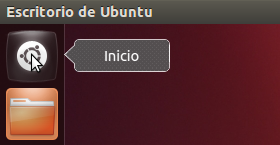
\includegraphics[width=0.45\textwidth]{ubuntu_boton_inicio}
    		}
    		\hfill
    		\subfloat[Buscador de Ubuntu\label{subfig:ubuntu_buscador}]%
    		{%
      		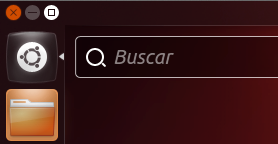
\includegraphics[width=0.45\textwidth]{ubuntu_buscador}
      	}
      	\hfill\centering
    		\subfloat[Icono del terminal de Ubuntu\label{subfig:ubuntu_terminal}]%
    		{%
      		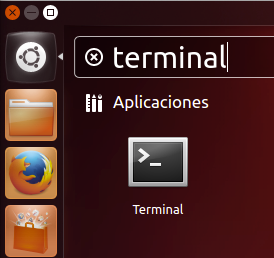
\includegraphics[width=0.4\textwidth]{ubuntu_terminal}
      	}
      	\caption{Apertura de un terminal en Ubuntu}
    		\label{fig:apertura_terminal_ubuntu}
    	\end{figure}

		\item Para instalar Flex escriba el siguiente comando en la terminal y pulse la tecla enter:

		\cod{sudo apt-get install flex}

		\fbox{\parbox{\linewidth}{\small Siempre que, durante la instalación de una herramienta, se le pregunte \pat{¿Desea continuar [S/n]?} escriba una \pat{S} mayúscula y pulse enter (figura~\ref{fig:ubuntu_instalacion_flex}).}}
		\begin{figure}[!ht]
			\centering
			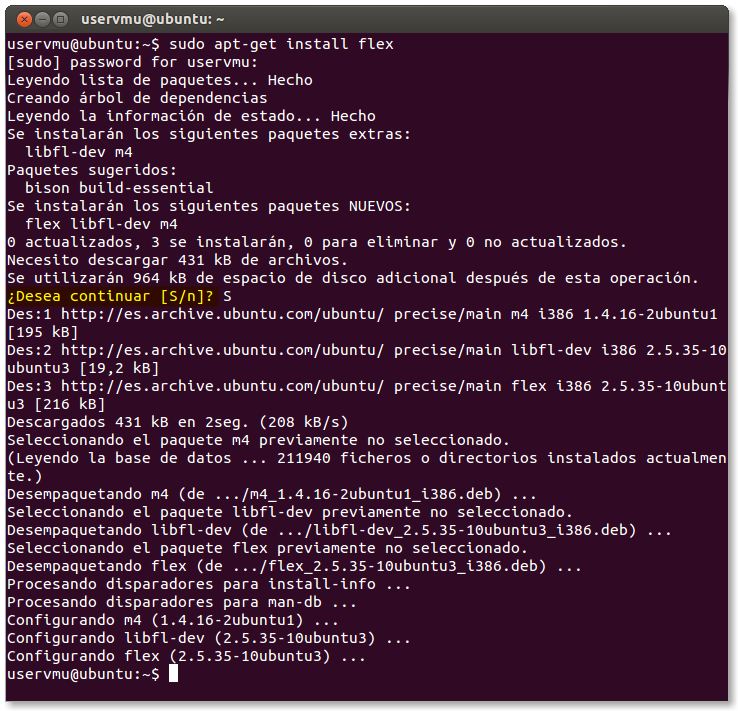
\includegraphics[width=0.85\textwidth]{ubuntu_instalacion_flex}
			\caption{Instalación de Flex en Ubuntu mediante el shell}
			\label{fig:ubuntu_instalacion_flex}
		\end{figure}

		\item Para instalar Bison escriba el siguiente comando y pulse enter:

		\cod{sudo apt-get install bison}

		\item Para instalar g++ escriba el siguiente comando y pulse enter:

		\cod{sudo apt-get install g++}

		\item La herramienta Make viene instalada por defecto en la mayoría de los sistemas basados en Linux. Si por casualidad su sistema no le proveyera dicha herramienta, puede utilizar el siguiente comando para instalarla:

		\cod{sudo apt-get install make}
	\end{enumerate}

	Otro modo de instalación es usando el centro de software de ubuntu.

\section{OS X}

	En los sistemas OS X puede obtener todas las herramientas necesarias instalando el IDE (entorno de desarrollo integrado) Xcode

	El IDE Xcode ocupa un espacio considerable (más de 5 GiB), puede obtener una instalación más liviana de las herramientas necesarias utilizando MacPorts \url{http://www.macports.org/ports.php?by=name&substr=gcc}

\section{Windows}


            %!TEX root = main.tex
\chapter{Instalación del compilador \Set}\label{app:installation_set_compiler}

	\section{Linux}


	\section{OS X}


	\section{Windows}

    % FIN del mainmatter
    %-----------------------------------------------------------------

  
    \backmatter% Este bloque contiene los anexos, bibliografía e índices alfabéticos. Se mantiene la misma numeración que en el mainmatter.

        \pdfbookmark[-1]{\bibname}{contents}% Añade la bibliogría a lista de marcadores y la coloca en el nivel -1, que es el nivel de una parte. De esta forma, el marcador de la bibliografía no que por debajo de la parte del apéndice.
        \hypersetup{bookmarksdepth=-2}% Desactiva los marcadores automáticos que se añaden con el paquete hyperref.
        \addcontentsline{toc}{chapter}{\bibname}
        \DeclareFieldFormat[inbook]{title}{\textit{#1}}% Establece a cursiva los títulos y subtítulos de los libros.
        \printbibliography% Imprime la entradas de la bibliografía (del archivo bibliography.bib).
    % FIN del backmatter
    %-----------------------------------------------------------------

\end{document}
% FIN del cuerpo
%***********************************************************************